\graphicspath{ {05-Source/Figures/} }

\section{Source}

A variety of options for the generation of the particle distribution
at source are included in the package (see section \ref{SourceOptions}).
The principal, and the default, option is the target-normal sheath
acceleration (TNSA) model presented in~\cite{10.1038/nphys199} .
The implementation of this model is summarised below.
The laboratory and RPLC reference frames coincide at the target,
therefore trace- and phase-coordinates are not distinguished in the
presentatiaon of the particle-production model.

\subsection{Energy distribution}

The typical kinetic energy spectrum produced in target-normal sheath
acceleration falls rapidly with kinetic energy before dropping rapidly
to zero above a maximum ``cut off'' energy $\varepsilon_{\rm max}$.
The kinetic-energy spectrum of the TNSA model presented
in~\cite{10.1038/nphys199} is given by:
\begin{equation}
  \frac{dN}{d\varepsilon} = \frac{n_{e0} c_{s} t_{laser} S_{sheath}}
                                 {\sqrt{2\varepsilon T_{e}}}
                                 \exp\left(
                                     - \sqrt{\frac{2\varepsilon}{T_{e}}}
                                     \right)\,;
  \label{Eq:Spct:0}
\end{equation}
where $N$ is the number of protons or ions produced per unit solid
angle, $\varepsilon$ is the ion kinetic energy, $n_{e0}$ and
$T_e$ are the hot electron density and temperature respectively, $c_s$
is the ion acoustic velocity, $t_{\rm laser}$ is the duration of the
laser pulse, and $S_{\rm sheath}$ is the effective area over which the
TNSA mechanism takes place.
The variables and the units in which they are expressed are presented
in table~\ref{table:EnergySpectrumParameters}.
\begin{table} 
  \caption{
    Parameters present in the analytical expression,
    equation \ref{Eq:Spct:0}, describing target normal sheath
    acceleration (TNSA).
  }
  \label{table:EnergySpectrumParameters}
  \begin{center}
    \begin{tabular}{c c c c}
      \hline
      \textbf{Parameter} & \textbf{Definition} & \textbf{Value} & \textbf{Unit} \\ [1ex] 
      \hline \hline
      $N$ & Ion number & - & - \\ 
      $\varepsilon$ & Ion kinetic energy & - & J \\  
      $n_{e0}$ & Hot electron density & $\frac{N_{E}}{c t_{laser} S_{sheath}}$ & $pp/m^3$ \\ 
      $N_{e}$ & Accelerated electron number & $\frac{f E_{laser}}{T_e}$ & - \\ 
      $E_{laser}$ & Laser energy & $70$ & J \\  
      $f$ & Energy conversion efficiency & $1.2 \times 10^{-15} I^{0.75}$, max=0.5  & - \\   % valid only for I < 3.1x10^19 W/cm2
      $I$ & Laser intensity & $4 \times 10^{20}$ & $W/cm^{2}$ \\ 
      $T_{e}$ & Hot electron temperature & $m_{e} c^{2} [\sqrt{1 + \frac{I \lambda^{2}}{1.37 \times 10^{18}} -1} ]$ & J \\ 
      $m_{e}$ & Electron mass & $9.11 \times 10^{-31}$ & Kg \\ 
      $c$ & Speed of light & $3 \times 10^{8}$ & m/s \\ 
      $\lambda$ & Laser wavelength & 0.8 & $\mu$m \\  
      $t_{laser}$ & Laser pulse duration & $28 \times 10^{-15}$  & s \\  
      $B$ & Radius of electron bunch & $B=r_{0} + d tan(\theta)$ & $m$ \\ 
      $S_{sheath}$ & Electron acceleration area & $\pi B^{2}$ & $m^{2}$ \\ 
      $r_{0}$ & Laser spot radius & $\sqrt{\frac{P_{laser}}{I \pi}}$, I in $W/m^{2}$ & m \\  
      $d$ & Target thickness & $400-600 \times 10^{-9}$ & m \\  
      $\theta$ & Electron half angle divergence & 0.436 & rad \\  
      $P_{laser}$ & Laser power & $2.5 \times 10^{15}$, $P_{laser}=\frac{E_{laser}}{t_{laser}}$ & W \\  
      $c_{s}$ & Ion-acoustic velocity & $(\frac{Z k_{B} T_{e}}{m_{i}})^{\frac{1}{2}}$ & m/s \\  
      $Z$ & Ion charge number & 1 & - \\  
      $k_{B}$ & Boltzmann constant & $1.380649 \times 10^{-23}$ & $m^{2} kg s^{-2} K^{-1}$ \\  
      $m_{i}$ & Proton mass & $1.67 \times 10^{-27}$ & Kg \\ 
      $P_{R}$ & Relativistic power unit & $\frac{m_{e} c^{2}}{r_{e}} = 8.71 \times 10^{9}$ & W \\  
      $r_{e}$ & Electron radius & $2.82 \times 10^{-15}$ & m \\  
      $\varepsilon_{i,\infty}$ & Maximum ion kinetic energy & $2 Z m_{e} c^{2} \sqrt{\frac{f P_{laser}}{P_{R}}}$ & MeV \\  
      $t_{0}$ & Ballistic time & $\frac{B}{v(\infty)}$ & s \\  
      $v(\infty)$ & Ballistic velocity & $\sqrt{\frac{2 \varepsilon_{i,\infty}}{m_{i}}}$ & m/s \\  
      \hline
    \end{tabular}
  \end{center}
\end{table}

Equation~\ref{Eq:Spct:0} is based on time-limited fluid-dynamical
models which are unable to predict the cut-off kinetic energy
accurately. 
The cut-off energy is taken to be that given by the model described
in~\cite{10.1103/PhysRevLett.97.045005} in which the time over which
the laser pulse creates the conditions necessary for acceleration is
derived.
The kinetic energy cut-off is given by:
\begin{equation}
  \varepsilon_{max} = X^{2} \varepsilon_{i,\infty} \, ;
  \label{eq:Eq:Spct:2}
\end{equation}
where $X$ is obtained by solving:
\begin{equation}
  \frac{t_{laser}}{t_{0}} = X \left( 1 + \frac{1}{2}
                           \frac{1}{1 - X^{2}} \right) +
                           \frac{1}{4} \ln \left( \frac{1+X}{1-X} \right) \, .
  \label{eq:Eq:Spct:1}
\end{equation}
Here $t_0$ is the time over which the ion acceleration may be treated
as ballistic and $\varepsilon_{i,\infty}$ is given in
table~\ref{table:EnergySpectrumParameters}.

To generate the kinetic energy spectrum, the probability density
function, $g(\varepsilon)$, is defined such that the probability,
$\delta {\cal P}$, of a particle being generated in the interval
$\varepsilon \rightarrow \varepsilon + \delta \varepsilon$ is given
by:
\begin{equation}
   \delta {\cal P} = g \left( \varepsilon \right) \delta \varepsilon \, .
\end{equation}
$g(\varepsilon)$ can be written in terms of the differential spectrum
given in equation~\ref{Eq:Spct:0} through the introduction of a
normalisation constant ${\cal N}$:
\begin{equation}
  g(\varepsilon) = \frac{1}{\cal N} \frac{dN}{d\varepsilon} \, .
\end{equation}
The cumulative distribution funtion, $G(\varepsilon)$, is given by:
\begin{equation}
  G(\varepsilon) = \int_{\varepsilon_{\rm min}}^{\varepsilon_{\rm max}} g(\varepsilon)
                                               d\varepsilon \,;
\end{equation}
where $\varepsilon_{\rm min}$ is the minimum kinetic energy and the
normalisation constant, ${\cal N}$, is set so that
$G(\varepsilon_{\rm max}) = 1$.
Carrying out the integration yields:
\begin{equation}
  G(\varepsilon) = \frac{2}{\cal N}
                   \frac{n_{e0} c_{s} t_{laser} S_{sheath}} {\sqrt{2T_{e}}}
                   \sqrt{\frac{T_{e}}{2}}
                   \left[
                         \exp\left(
                                   -\sqrt{\frac{2\varepsilon_{\rm min}}{T_{e}}}
                             \right) -
                         \exp\left(
                                   -\sqrt{\frac{2\varepsilon}{T_{e}}}
                             \right)
                   \right] \, ;
\end{equation}
and the normalisation constant is given by:
\begin{equation}
  {\cal N} = 2
             \frac{n_{e0} c_{s} t_{laser} S_{sheath}} {\sqrt{2T_{e}}}
             \sqrt{\frac{T_{e}}{2}}
             \left[
                   \exp\left(
                             -\sqrt{\frac{2\varepsilon_{\rm min}}{T_{e}}}
                             \right) -
                         \exp\left(
                                   -\sqrt{\frac{2\varepsilon}{T_{e}}}
                              \right)
             \right] \, .
\end{equation}

The kinetic energy spectrum may now be obtained by choosing a value
for $G(\varepsilon)$ using a probability distribution uniform over the
range $0 < G(\varepsilon) < 1$.
The generated value of $\varepsilon$ is obtained by evaluating:
\begin{equation}
  \varepsilon = \left[
                      \sqrt{\varepsilon_{\rm min}} -
                      \sqrt{\frac{T_e}{2}} \ln \left(
                     1 - \frac{G(\varepsilon)}{G(\varepsilon_{\rm max})}
                                               \right)
                \right]^2 \, .
\end{equation}

\subsection{Angular Distribution}

The angular distribution of the flux of protons and ions produced by
the TNSA mechanism may be described as a cone centred on the normal to
the foil surface~\cite{10.1063/1.3086424}.
Radiochromic film has been used to observe the opening angle,
$2\alpha$, of the cone as a function of energy.
The envelope angle, $\alpha$, defined such that, at a particular
energy, all particles are contained within $\pm\alpha(\varepsilon)$ of
the $z$ axis.
The opening angle is observed to decrease as the ion energy
increases.

The distribution of the polar angle, $\theta_S$, at which particles
are produced at the laser-driven source is generated by defining
$r^\prime$ such that:
\begin{equation}
  r^\prime = \frac{\partial r}{\partial s}\,;
\end{equation}
where $r=\sin\theta_S$.
$x^\prime$ and $y^\prime$ are sampled independently from the
probability density function:
\begin{equation}
  g(r^\prime) = \frac{3}{4r^{\prime 2}_m} \left(r^{\prime 2}_m-r^{\prime 2} \right)\,;
\end{equation}
where $r^\prime_m=\sin\alpha$.
At low kinetic energy ($\varepsilon \sim \varepsilon_{\rm min}$),
$\alpha(\varepsilon)$ is taken to be $\sim 20^\circ$.
$\alpha(\varepsilon)$ is assumed to decrease linearly with energy such
that:
\begin{equation}
  \alpha(\varepsilon) =
                20^\circ - 15^\circ \frac{\varepsilon}{\varepsilon_{max}} \, ;
  \label{Eq:sigVeps}
\end{equation}
i.e. $\alpha(\varepsilon)$ decreases from $20^\circ$ at $\varepsilon=0$
to $5^\circ$ at $\varepsilon_{max}$.
Finally, the azimuthal angle, $\phi_S$, is chose from a distribution
uniform over the range $0 < \phi_S < 2\pi$.

\subsection{Spatial distribution}

The $x$ and $y$ distributions at production are assumed to be
independent and Gaussianly distributed with a standard deviation given
by the radius of the laser spot focused on the target.

\begin{figure}
  \begin{center}
    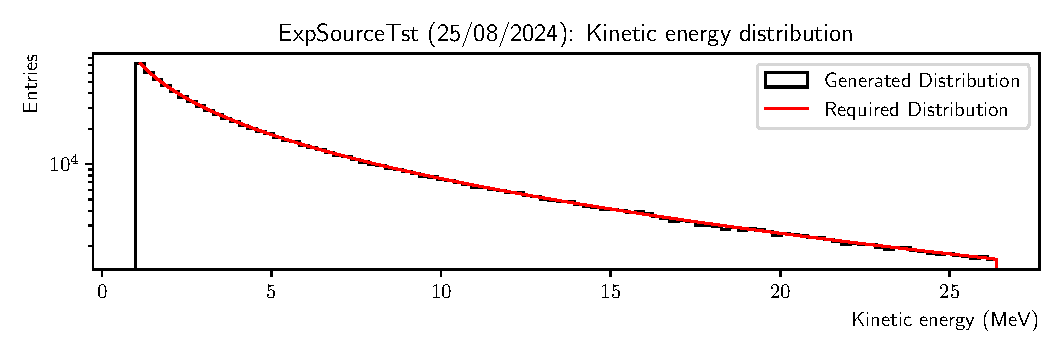
\includegraphics[width=0.92\linewidth]{SourceTst_K.pdf}
    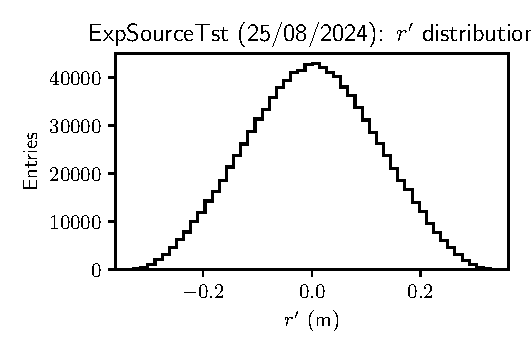
\includegraphics[width=0.46\linewidth]{SourceTst_rp.pdf}
    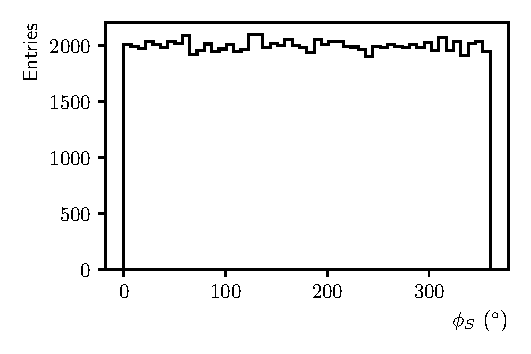
\includegraphics[width=0.46\linewidth]{SourceTst_phi.pdf}
    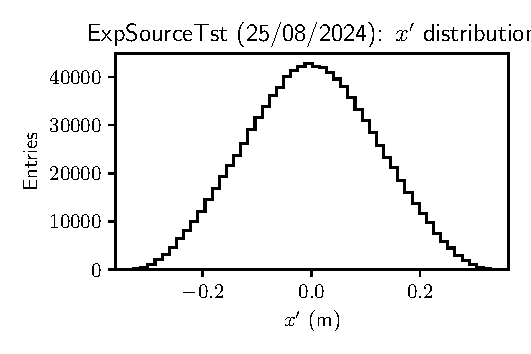
\includegraphics[width=0.46\linewidth]{SourceTst_xp.pdf}
    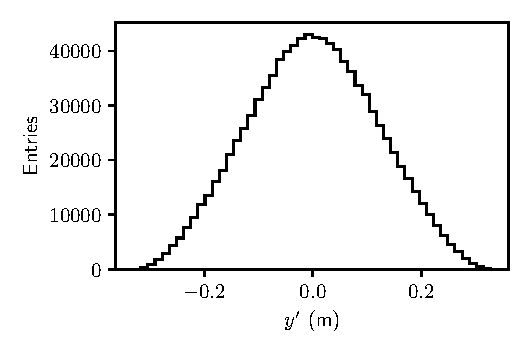
\includegraphics[width=0.46\linewidth]{SourceTst_yp.pdf}
    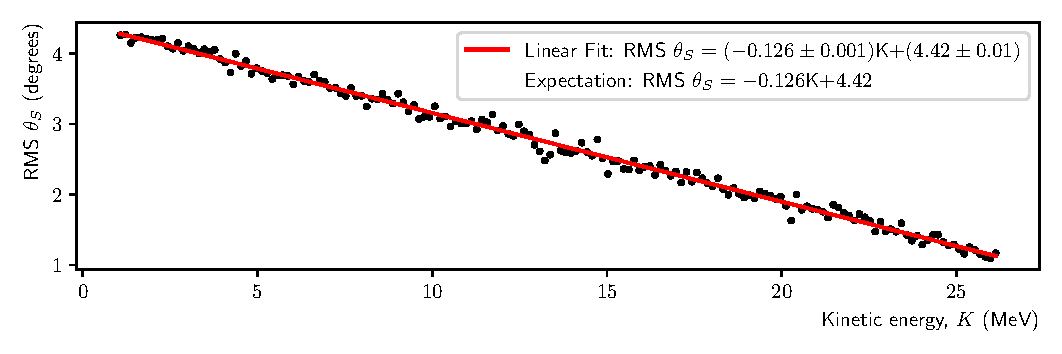
\includegraphics[width=0.92\linewidth]{RMS_Set_kE.pdf}
  \end{center}
  \caption{Kinematic distributions of particles at the point of
    production.
    \underline{Top:} The generated kinetic energy disribution is shown
    as the solid histogram. 
    The required distribution (equation~\ref{Eq:Spct:0}), normalised
    to the lowest kinetic-energy bin, is shown as the solid red line.
    \underline{Second row:} Generated $r^\prime$ and $\phi_S$
    distributions. 
    \underline{Third row:} Generataed $x^\prime$ and $y^\prime$
    distributions. 
    \underline{Bottom:} RMS of the $\theta_S$ distribution versus
    kinetic energy.
    The solid circles are calculated using slices of width 0.15\,MeV.
    The red line shows the result of a straight line fit to the data.
    The expected dependence from integration of
    equation~\ref{Eq:sigVeps} is presented in the legend.
  }
  \label{Fig:LsrDrvSrc:Dists}
\end{figure}

\begin{figure}
  \begin{center}
    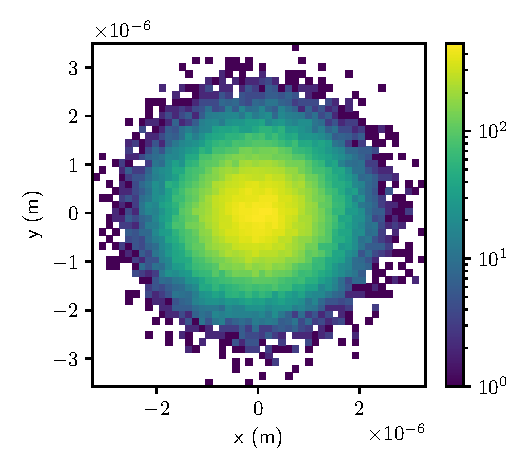
\includegraphics[width=0.46\linewidth]{SourceTst_xy.pdf}
    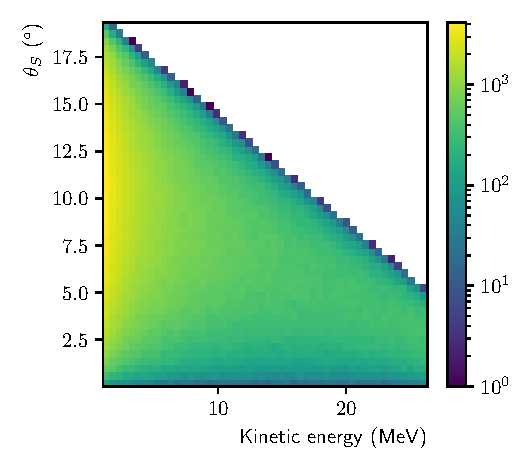
\includegraphics[width=0.46\linewidth]{SourceTst_thetaK.pdf}
    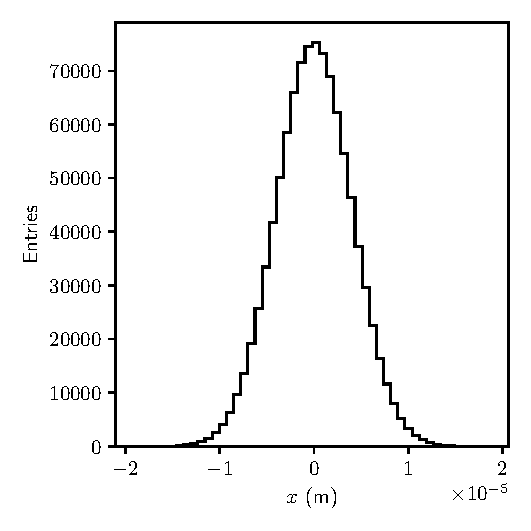
\includegraphics[width=0.46\linewidth]{SourceTst_x.pdf}
    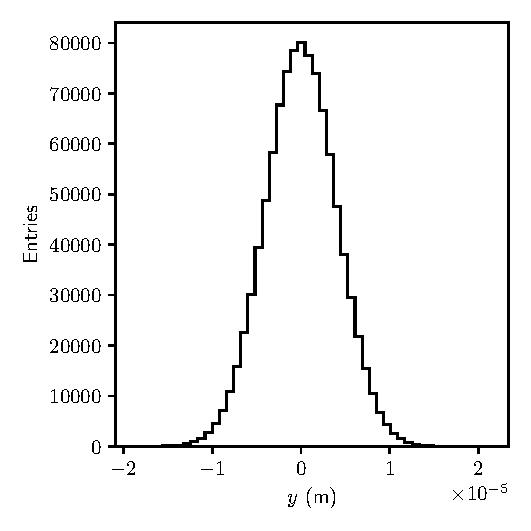
\includegraphics[width=0.46\linewidth]{SourceTst_y.pdf}
    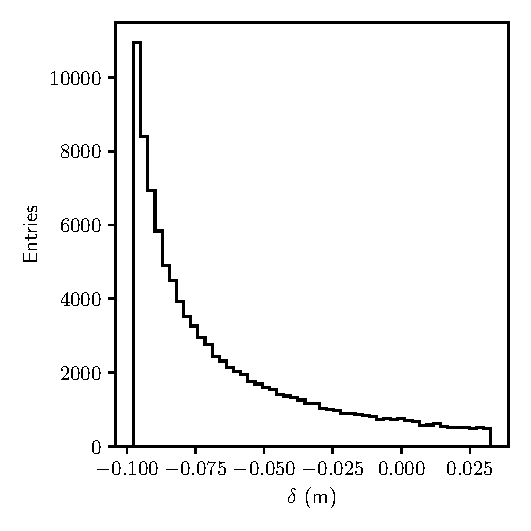
\includegraphics[width=0.46\linewidth]{SourceTst_d.pdf}
    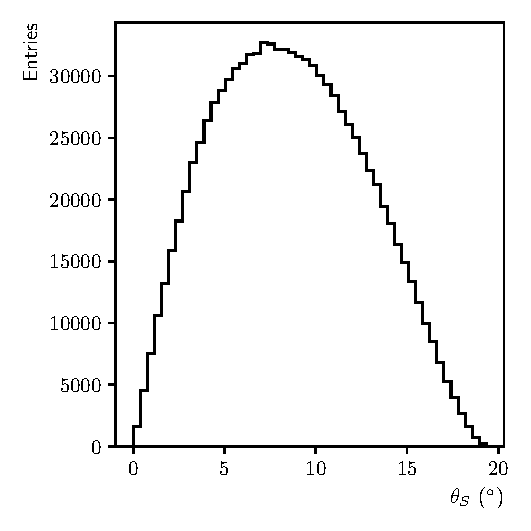
\includegraphics[width=0.46\linewidth]{SourceTst_theta.pdf}
  \end{center}
  \caption{
    \underline{Top left:} Generated $(x, y)$ distribution of the
    particle-production point.
    \underline{Top right:} The distribution of $\theta_S$ versus
    kinetic energy.
    \underline{Centre left, right:} Gemerated disributions of
    $x^\prime$ and $y^\prime$.
    \underline{Bottom left:} Generated distribution of $\delta$.
    \underline{Bottom right:} Generated distribution of $\theta_S$.
  }
  \label{Fig:LsrDrvSrc:Dists}
\end{figure}

\subsection{Simulated distributions}

Distributions $10^6$ protons produced by the TNSA mechanism using the
algorithm described above are shown in
figure~\ref{Fig:LsrDrvSrc:Dists}.
The parameters used in the algorithm are presented in
table~\ref{Tab:Src:Param}.
The generated distribution of kinetic energy is in good agreement with
the distribution implied by equation~\ref{Eq:Spct:0}.
The width of the generated polar-angle distribution is observed to
fall with kinetic energy and the kinetic-energy dependence of the RMS
calculated from the generated particles is in good agreement with that
expected from equation~\ref{Eq:sigVeps}.
As a result, the distribution of $\theta_S$ is approximately Gaussian
with a width dominated by the contribution of protons with kinetic
energy close to $\varepsilon_{\rm min}$.
The generated $\phi_S$ distribution is flat in the range
$0^\circ < \phi_S < 360^\circ$ and the $(x, y)$ distribution is
Gaussian in both the $x$ and $y$ projections.
\begin{table}
  \caption{Parameterised laser driven}
  \label{Tab:Src:Param}
  \begin{center}
    \begin{tabular}{|l|c|l|}
      \hline
        \textbf{Parameter} & \textbf{Value} & \textbf{Unit} \\ 
        \hline
        $\sigma_x$&4e-06&$\mu$m \\ 
        $\sigma_y$&4e-06&$\mu$m \\ 
        $\cos\theta_S |_{\rm min}$&0.998& \\ 
        $\varepsilon_{\rm min}$&1.0&MeV \\ 
        $\varepsilon_{\rm max}$&25.0&MeV \\ 
        nPnts&1000& \\ 
        Laser power&2500000000000000.0&W \\ 
        Laser energy&70.0&J \\ 
        Laser wavelength&0.8&$\mu$m \\ 
        Laser pulse duration&2.8e-14&s \\ 
        Laser spot size&4e-07&$\mu$m \\ 
        Laser intensity&4e+20&J$/m^2$ \\ 
        Electron divergence angle&25.0&degrees \\
        RMS $\theta_S$ at $K=0$\,MeV & 20 & degrees \\
        Scaled slope of RMS $\theta_S$ versus $K$ & 15 & degrees \\
      \hline
    \end{tabular}
  \end{center}
\end{table}
